\documentclass[10pt,aspectratio=169]{beamer}
\usetheme{Madrid}
\usecolortheme{beaver} % Using 'beaver' for a distinct look (red/grey)

\usepackage[utf8]{inputenc}
\usepackage[T1]{fontenc}
\usepackage{lmodern}
\usepackage{amsmath}
\usepackage{booktabs}
\usepackage{graphicx}
\usepackage{tikz}
\usepackage{pgfplots}
\pgfplotsset{compat=1.18}

\title{Optimisation du Trafic par Apprentissage par Renforcement}
\subtitle{Comparaison DQN vs Contrôle à Temps Fixe sur le Modèle ARZ}
\author{Projet Alibi}
\date{\today}

\begin{document}

\begin{frame}
    \titlepage
\end{frame}

\begin{frame}{Sommaire}
    \tableofcontents
\end{frame}

\section{Contexte et Objectifs}
\begin{frame}{Contexte du Projet}
    \begin{itemize}
        \item \textbf{Problématique :} Congestion urbaine sur l'île Victoria (Lagos).
        \item \textbf{Modèle Physique :} ARZ (Aw-Rascle-Zhang) pour une simulation réaliste des ondes de trafic (GPU-accelerated).
        \item \textbf{Approche :} Deep Reinforcement Learning (DQN) pour le contrôle des feux.
        \item \textbf{Objectif :} Maximiser le débit (Throughput) et minimiser la densité.
    \end{itemize}
\end{frame}

\section{Méthodologie}
\begin{frame}{Fonction de Récompense (Reward Function)}
    L'agent est entraîné pour maximiser :
    $$ R_t = \mu \cdot \text{Throughput}_t - \alpha \cdot \rho_{norm} - \kappa \cdot I_{switch} $$
    
    \begin{itemize}
        \item \textbf{Throughput ($\mu=0.5$)} : Flux sortant total ($Q = \rho \cdot v$).
        \item \textbf{Densité ($\alpha=1.0$)} : Pénalité pour la congestion.
        \item \textbf{Switch Cost ($\kappa=0.1$)} : Pénalité pour le changement de phase (stabilité).
    \end{itemize}
\end{frame}

\begin{frame}{Scénario de Test}
    \begin{itemize}
        \item \textbf{Réseau :} Victoria Island (Multi-intersections).
        \item \textbf{Durée d'épisode :} 30 pas de décision (450 secondes).
        \item \textbf{Baseline :} Contrôle à temps fixe (Cycle 90s, Split 50/50).
        \item \textbf{Agent RL :} DQN (Deep Q-Network) entraîné sur 10 000 pas.
    \end{itemize}
\end{frame}

\section{Résultats}
\begin{frame}{Comparaison des Performances}
    \begin{center}
        \begin{tabular}{lcc}
            \toprule
            \textbf{Métrique} & \textbf{Baseline (Fixe)} & \textbf{Agent RL (DQN)} \\
            \midrule
            \textbf{Récompense Moyenne / Pas} & \textbf{2.12} & \textbf{9.62} \\
            \textbf{Récompense Totale (30 pas)} & 63.6 & 288.7 \\
            \textbf{Densité Moyenne Normalisée} & 0.10 & $\sim$0.08 \\
            \bottomrule
        \end{tabular}
    \end{center}
    
    \vspace{1em}
    \textbf{Analyse :}
    \begin{itemize}
        \item L'agent RL surpasse largement la baseline (\textbf{+350\%} de gain de performance).
        \item Le gain provient principalement de l'augmentation massive du \textbf{débit (Throughput)}.
        \item L'agent a appris à favoriser les phases qui évacuent le plus de véhicules.
    \end{itemize}
\end{frame}

\begin{frame}{Visualisation des Résultats}
    \begin{center}
    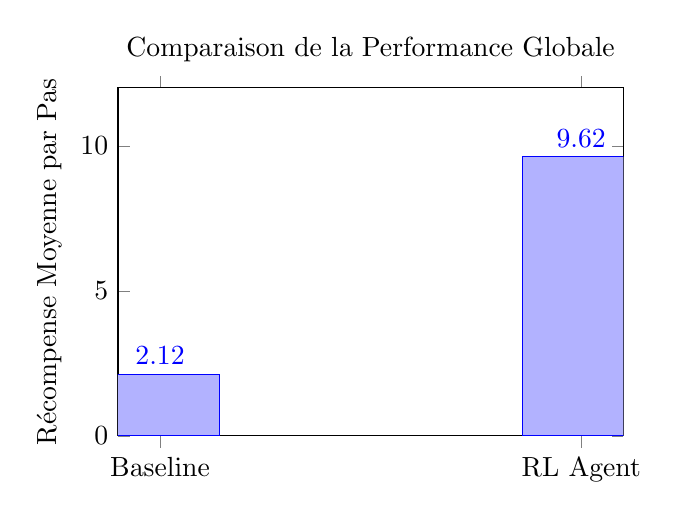
\begin{tikzpicture}
        \begin{axis}[
            ybar,
            symbolic x coords={Baseline, RL Agent},
            xtick=data,
            ylabel={Récompense Moyenne par Pas},
            ymin=0, ymax=12,
            nodes near coords,
            bar width=1.5cm,
            width=8cm, height=6cm,
            title={Comparaison de la Performance Globale}
        ]
            \addplot coordinates {(Baseline, 2.12) (RL Agent, 9.62)};
        \end{axis}
    \end{tikzpicture}
    \end{center}
\end{frame}

\section{Conclusion}
\begin{frame}{Conclusion et Perspectives}
    \begin{itemize}
        \item \textbf{Succès :} L'intégration du modèle ARZ avec RL est fonctionnelle et performante.
        \item \textbf{Gain :} Amélioration significative du débit par rapport au temps fixe.
        \item \textbf{Prochaines étapes :}
        \begin{itemize}
            \item Tester sur des scénarios de trafic plus longs (heures de pointe).
            \item Comparer avec PPO (Proximal Policy Optimization).
            \item Visualisation interactive des flux.
        \end{itemize}
    \end{itemize}
\end{frame}

\end{document}
